% Created 2013-12-14 Sat 15:44
\documentclass[]{article}
\usepackage[utf8]{inputenc}
\usepackage[T1]{fontenc}
\usepackage{fixltx2e}
\usepackage{graphicx}
\usepackage{longtable}
\usepackage{float}
\usepackage{wrapfig}
\usepackage{rotating}
\usepackage[normalem]{ulem}
\usepackage{amsmath}
\usepackage{textcomp}
\usepackage{marvosym}
\usepackage{wasysym}
\usepackage{amssymb}
\usepackage{hyperref}
\tolerance=1000
\usepackage{amsfonts,amssymb,amsmath,amsthm,bm}
\author{Daniele Barchiesi and Mark D. Plumbley}
\date{\textit{<2013-12-13 Fri>}}
\title{Classification via dictionary learning: incoherent sub-space modelling for high-dimensional data}
\hypersetup{
  pdfkeywords={},
  pdfsubject={},
  pdfcreator={Emacs 24.3.1 (Org mode 8.2.4)}}
\begin{document}

\maketitle
/Users/daniele/Dropbox/Career/Research/MyPapers/Projects/2013-MLSP/definitions.tex

\begin{abstract}

\end{abstract}

\section{Introduction}
\label{sec-1}
\subsection{Problem definition}
\label{sec-1-1}
\subsection{Previous work and applications}
\label{sec-1-2}

\subsection{Outline and main contributions}
\label{sec-1-3}

\section{Background}
\label{sec-2}
\subsection{Benchmark techniques}
\label{sec-2-1}
\subsubsection{Features transform for classification}
\label{sec-2-1-1}
Feature transforms have been used to model data in an attempt to enhance the tradeoff between generalisation and discrimination, as described in Section \ref{sec-1}.

Two of the most common feature transform techniques include principal component analysis (PCA) \cite{Pearson1901On} and Fisher's linear discriminant analysis (LDA) \cite{Duda1973Pa}. This section provides a brief description of their rationale.

Let $\{\Vector{x}_m \in \real^N\}$ be a set of vectors containing features extracted from $M$ training signals.
\subsection{Manifold learning}
\label{sec-2-2}
\subsection{Dictionary learning}
\label{sec-2-3}
\subsubsection{Dictionary learning for sparse approximation}
\label{sec-2-3-1}
\subsubsection{Incoherent dictionary learning}
\label{sec-2-3-2}
\subsubsection{Dictionary learning for classification}
\label{sec-2-3-3}

\section{Learning incoherent subspaces using iterative projections and rotations}
\label{sec-3}
\section{Numerical Experiments}
\label{sec-4}
This is an experimental image that describes our results.
RESULTS:



\begin{figure}[htb]
\centering
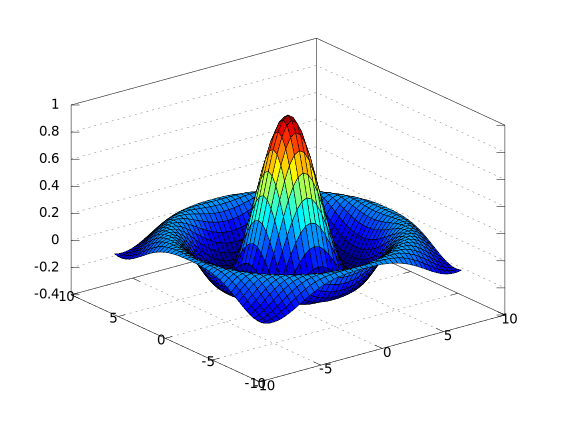
\includegraphics[width=.9\linewidth]{./images/chart.pdf}
\caption{\label{fig:SED-HR4049}This is the caption for the next figure link (or table)}
\end{figure}
\section{Discussion}
\label{sec-5}
\section{Conclusions}
\label{sec-6}

\bibliographystyle{plain}
\bibliography{/Users/daniele/Dropbox/Career/Research/MyPapers/bibliography.bib}
% Emacs 24.3.1 (Org mode 8.2.4)
\end{document}
